\documentclass[11pt]{article}
\usepackage{tikz}
\usetikzlibrary{calc}
\usepackage{eso-pic}
\usepackage{hyperref}
\usepackage{listings}
\usepackage{enumitem}
\usepackage{amsmath}
\usepackage{xepersian}
\usepackage{lipsum}
\usepackage{xcolor}
\usepackage{listings}
\settextfont[]{Niloofar.ttf}
\usepackage[english]{babel}
\usepackage[utf8x]{inputenc}
\usepackage{graphicx}
\usepackage[colorinlistoftodos]{todonotes}
\usepackage{filecontents}
\usepackage{verbatim}
\usepackage{eurosym}
\usepackage[export]{adjustbox}


\hypersetup{
  colorlinks, linkcolor=red
}
\AddToShipoutPictureBG{%
\begin{tikzpicture}[overlay,remember picture]
\draw[line width=4pt]
    ($ (current page.north west) + (1cm,-1cm) $)
    rectangle
    ($ (current page.south east) + (-1cm,1cm) $);
\draw[line width=1.5pt]
    ($ (current page.north west) + (1.2cm,-1.2cm) $)
    rectangle
    ($ (current page.south east) + (-1.2cm,1.2cm) $);
\end{tikzpicture}
}

\begin{document}

\begin{titlepage}

\newcommand{\HRule}{\rule{\linewidth}{0.5mm}}

\center 

\textsc{\LARGE به نام خدا}\\[1.5cm] 


\textsc{\Large درس امنیت سیستم‌های کامپیوتری}\\[0.5cm] 

\HRule \\[0.4cm]
{ \huge \bfseries پروژه ایریدیم}\\[0.4cm] 
\HRule \\[1.5cm]

\begin{minipage}{0.4\textwidth}
\begin{flushright} \large
\emph{دانشجویان:}\\
 محمد اصولیان\\
  پوریا رحیمی\\
\end{flushright}
\end{minipage}
~
\begin{minipage}{0.4\textwidth}
\begin{flushright} \large
\emph{مدرس درس: } \\
دکتر ابوالفضل دیانت \\
\end{flushright}
\end{minipage}\\[2cm]

\end{titlepage}

\newpage
\section{مقدمه}
پروژه ایریدیم، یک شبیه سازی از بدافزار معروف میرای(Mirai) است که در سال 2016 توانست با آلوده کردن هزاران دستگاه و ارسال درخواست DNS به سرور Dyn، این سرور را مختل و دسترسی بسیاری از وبسایت‌های معروف در جهان را مختل کنید.

\section{شرح پروژه}
هدف این پروژه نوشتن برنامه‌ای است که با اسکن شبکه، پورت‌های باز شبکه را کشف کرده و در صورتی که روی این پورت‌ها سرویس ssh اجرا می‌شد، با تست کردن پسوردهای معروف، به این کامپیوترها نفوذ کرده و بدافزاری را روی آنها بارگذاری کند که اطلاعات امنیتی سیستم را جمع آوری و در زمان های مشخص به یک وب سرور مشخص ارسال می‌کند.

\section{ساختار پروژه}

این پروژه روی محیط شبیه سازی شده در داکر اجرا می‌شود. به کمک داکر می‌توان یک شبکه داکر ایجاد کرد و تعدادی container به آن اضافه کرد و سپس حمله را در این شبکه شبیه‌سازی کرد. در این شبکه از سه نوع image سرور هدف، وب سرور و سیستم حمله کننده برای شبیه سازی استفاده شده که در ادامه شرح داده خواهند شد.

\subsection{targe-server}
سرورهای قربانی سرورهایی هستند که حمله به آنها صورت می‌گیرد. image این سرورها روی لینوکس alpine قرار گرفته که تا جای امکان سبک باشند. همچنین برای اجرای بهتر شبیه سازی، برخی سرویس‌ها مانند ssh و ftp روی این سرورها نصب شده.

\subsection{web-server}
این وب سرور کوچک به کمک فریم‌ورک django با اهداف زیر پیاده‌سازی شده:


\begin{itemize}
    \item دانلود بدافزار توسط سرورهای قربانی از این وب سرور.
    \item ارسال اطلاعات امنیتی جمع‌آوری شده از قربانی‌ها برای این وب سرور.
    \item ذخیره اطلاعات جمع‌آوری شده در یک دیتابیس.
	\item طراحی یک رابط کاربری ساده برای مشاهده دیتابیس و امکان حذف، مرتب‌سازی و ویرایش اطلاعات.
\end{itemize}

دوتا از دلایل مهم استفاده از فریم‌ورک django برای این وب سرور، وجود پنل ادمین در این فریم‌ورک و امکان استفاده از دیتابیس‌های سبک sqlite بود.

در این وب سرور یک اسکریپت به نام infogather.sh ذخیره شده که با get کردن، روی سرور قربانی دانلود و ذخیره می‌شود. این اسکریپت اطلاعات مهم و امنیتی کامپیوتر را در قالب یک فایل json، برای وب سرور ارسال می‌کند. نمونه این اطلاعات را می‌توانید در دیتابیس وبسرور مشاهده کنید.

\begin{figure}[hbtp]
\caption{نمونه فیلدهای استخراج شده از سرورهای قربانی}
\centering
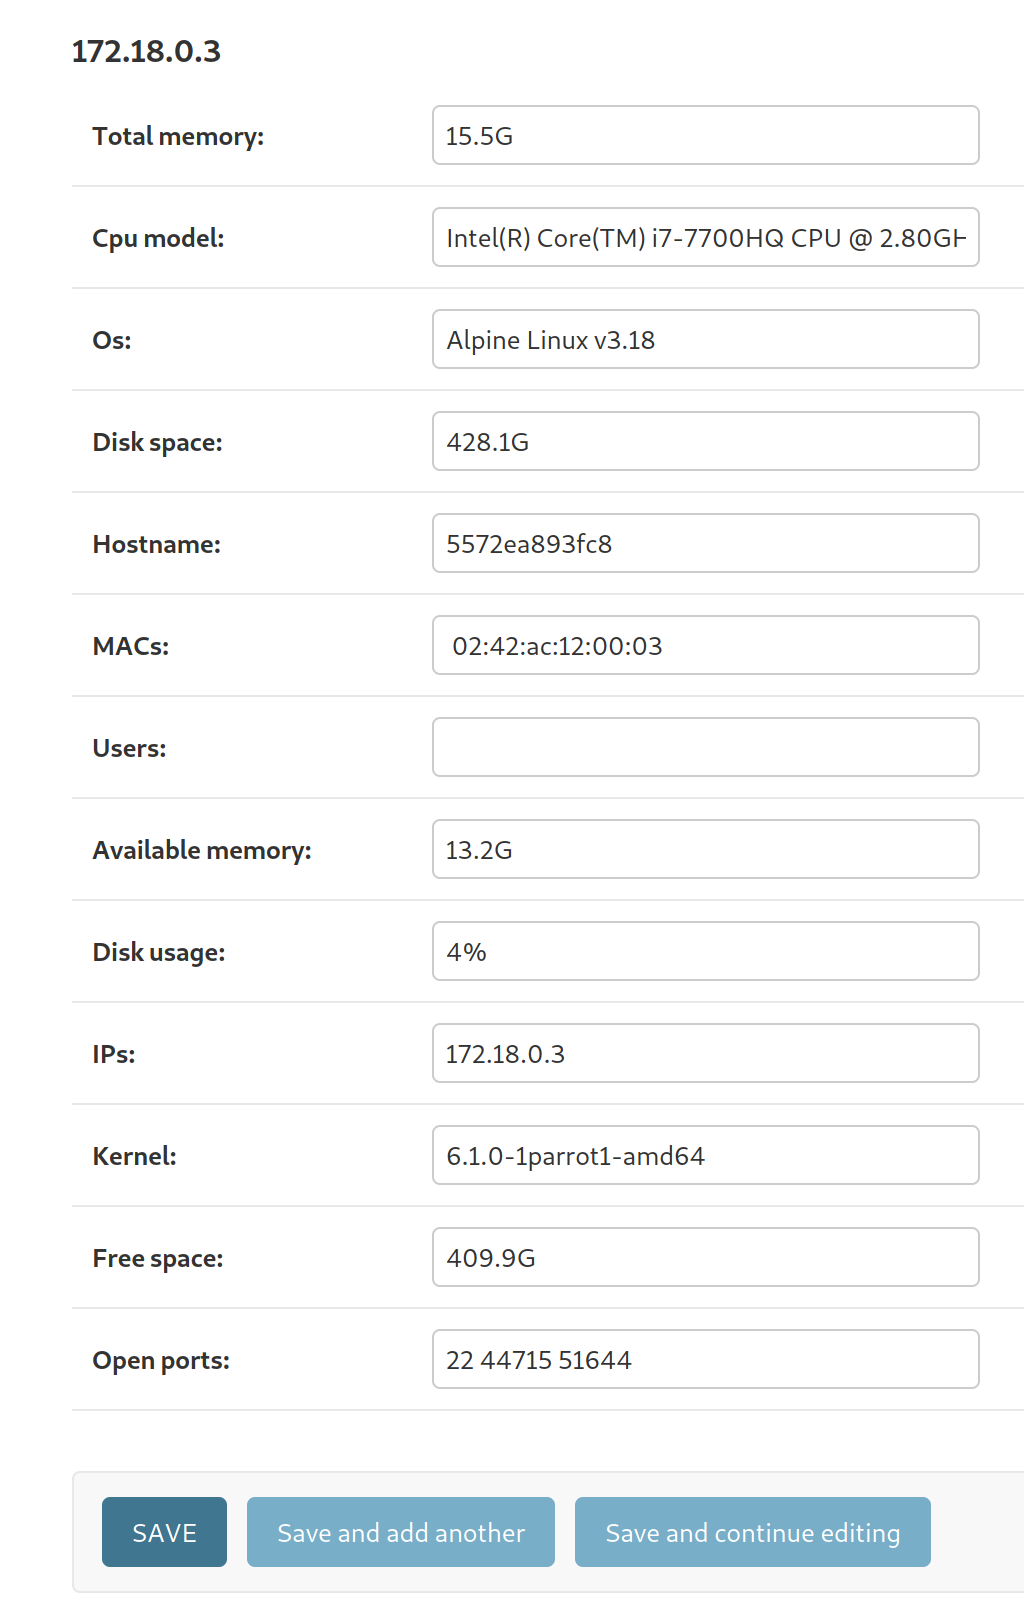
\includegraphics[scale=0.2]{images/host_security_info.png}
\end{figure}


برای محرمانه ماندن ارتباطات بین این وب سرور و سرورهای قربانی، ارتباطات از طریق پروتکل https انجام می‌شود که رمزنگاری شده و امن است.

\subsection{attacker-machine}
در نهایت، برای حمله به سرورهای قربانی، یک image برای سیستم حمله کننده ایجاد شد. این image هم از لینوکس alpine گرفته شده که تا حد امکان سبک باشد. همچنین ابزارهای لازم برای حمله مانند nmap و nc و curl و ssh client و ... روی این ماشین نصب شده و اسکریپت‌های اسکن و حمله هم روی image قرار داده شد تا به محض بالا آمدن container، بتوان از این سیستم استفاده کرد.

فایل‌های قرار داده شده در این image به شرح زیر هستند:
\begin{itemize}
    \item[scan.sh] این اسکریپت یک رینج ip را در ورودی دریافت می‌کند و تمام هاست‌های فعال در این رینج را بررسی کرده و پورت‌های باز آنها را پیدا می‌کند. سپس اطلاعات پیدا شده را در فایلی به نام open\_ports با فرمت csv ذخیره می‌کند.
    \item[hack.sh] این اسکریپت اطلاعات را از روی فایل open\_ports.csv می‌خواند و به پورت‌های ssh یافت شده حمله می‌کند. حمله به صورت تست کردن رمزعبورهای پرتکرار انجام می‌شود. در صورتی که اتصال با سرور قربانی برقرار شد، بدافزار از وب سرور بر روی سرورقربانی دانلود و اجرا می‌شود. لازم است که ip وب سرور حین اجرای این اسکریپت به عنوان ورودی به آن داده شود.
    \item[userpass.csv] در این فایل، user و password های پرتکرار ذخیره شده که در حمله به ssh استفاده می‌شوند.
\end{itemize}



برای هر کدام از این image ها یک dockerfile نوشته شده. از image سرور هدف، چندین کانتینر اجرا می‌شود و از image سیستم حمله کننده و وب سرور تنها یک کانتینر اجرا می‌شود.

\section{اسکریپت‌های کمکی}
برای اجرای پروژه چند اسکریپت کمکی هم نوشته شده که فرایند ساخت و اجرای داکرفایل‌ها را سریع‌تر و راحت‌تر می‌کند. همه این اسکریپت‌ها در root پروژه موجود هستند و در ادامه توضیح داده می‌شوند.

\subsection{build\_image.sh}
با اجرای این اسکریپت، image ها از روی داکرفایل‌ها به صورت خودکار ایجاد می‌شوند.

\subsection{setup\_sim.sh}
    با اجرای این اسکریپت، ابتدا یک شبکه داکر ایجاد شده و سپس image های ساخته شده به صورت خودکار در آن شبکه اجرا می‌شوند
    
\subsection{remove\_containers.sh}
با اجرای این اسکریپت، continer های ایجاد شده متوقف و حذف می‌شوند.

\section{تست پروژه}
برای اجرای پروژه و تست درستی آن مراحل ذیل را دنبال کنید.

\subsection{اجرای container ها}
برای راه‌اندازی شبکه، ابتدا اسکریپت build\_images.sh را اجرا کنید تا image ها ساخته شوند. سپس اسکریپت setup\_sim.sh را اجرا کنید تا container ها اجرا شوند.

\begin{figure}[hbtp]
\caption{راه‌اندازی شبکه داکر به کمک اسکریپت srtup\_sim.sh}
\centering
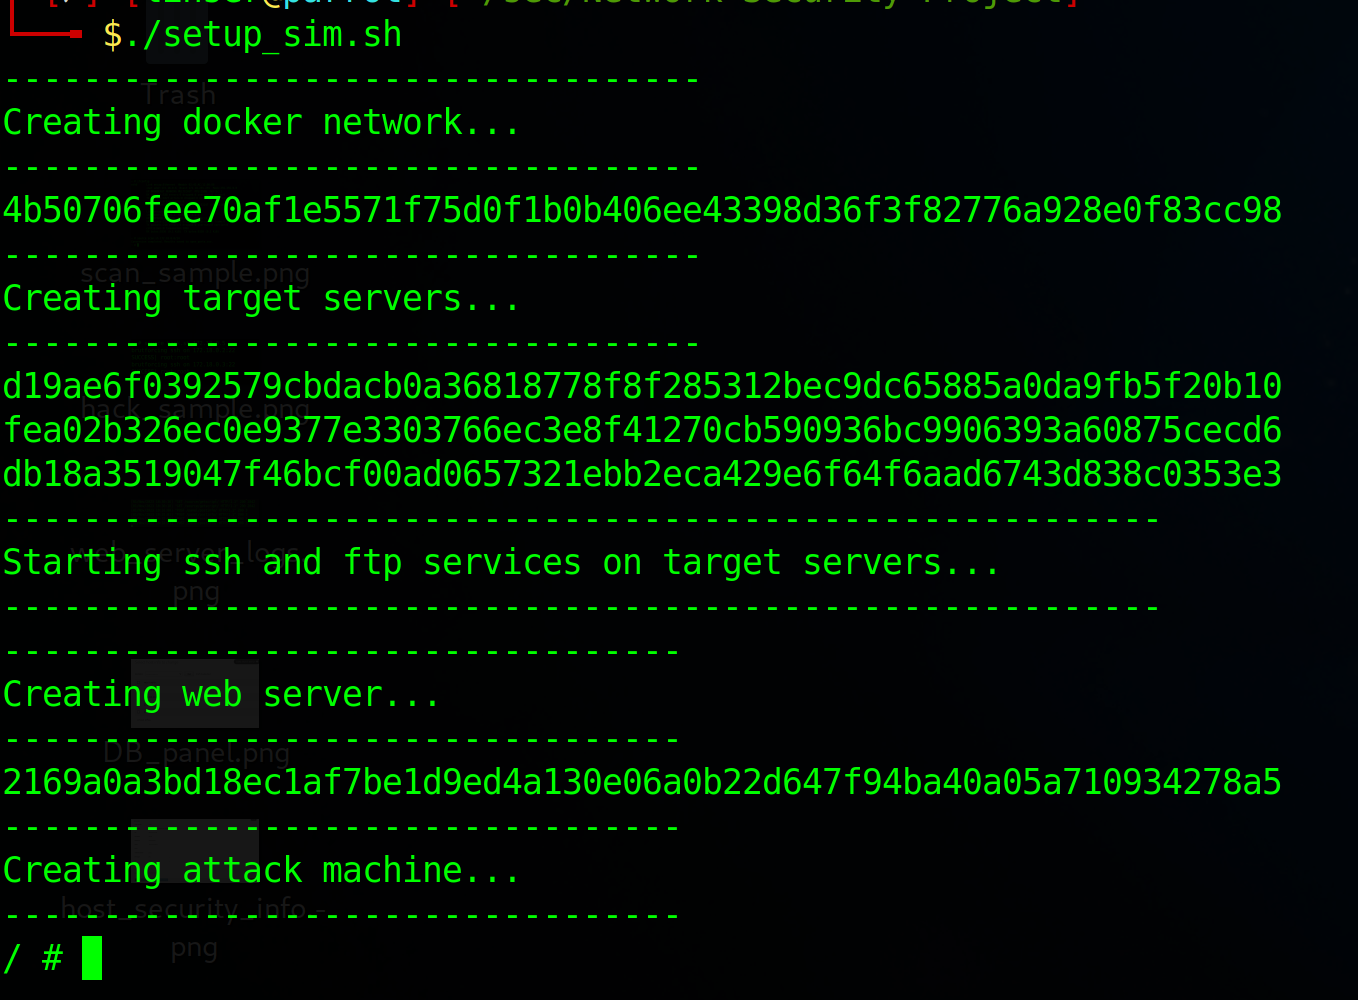
\includegraphics[scale=0.2]{images/setup_sim.png}
\end{figure}


پس از اجرای اسکریپت setup\_sim.sh، یک ترمینال به شما در سیستم attacker داده می‌شوند تا حمله را شروع کنید.


همچنین وب سرور روی پورت 8000 در لوکال‌هاست شما قابل مشاهده است. برای مشاهده دیتابیس این وب سرور به صفحه \url{127.0.0.1:8000/admin} مراجعه کنید. توجه داشته باشید که نام کاربری و پسورد ورود به این صفحه، superuser:superuser می‌باشد.


\subsection{حمله به سرورهای هدف}
ابتدا با اجرای دستور ifconfig یا با استفاده از دستورات داکر، آدرس نتورک شبکه داکر که کانتینرهای در آن در حال اجرا هستند را پیدا کنید. سپس فایل scan.sh را اجرا کرده و رینج مدنظر برای اسکن را به صورت NETWORK\_ADDRESS/24 به آن ورودی بدهید. پس از اتمام اسکن، نتایج در فایل open\_ports.csv برای شما قابل مشاهده هستند.

\begin{figure}[hbtp]
\caption{پیدا کردن نتورک آدرس و اجرای اسکریپت scan.sh}
\centering
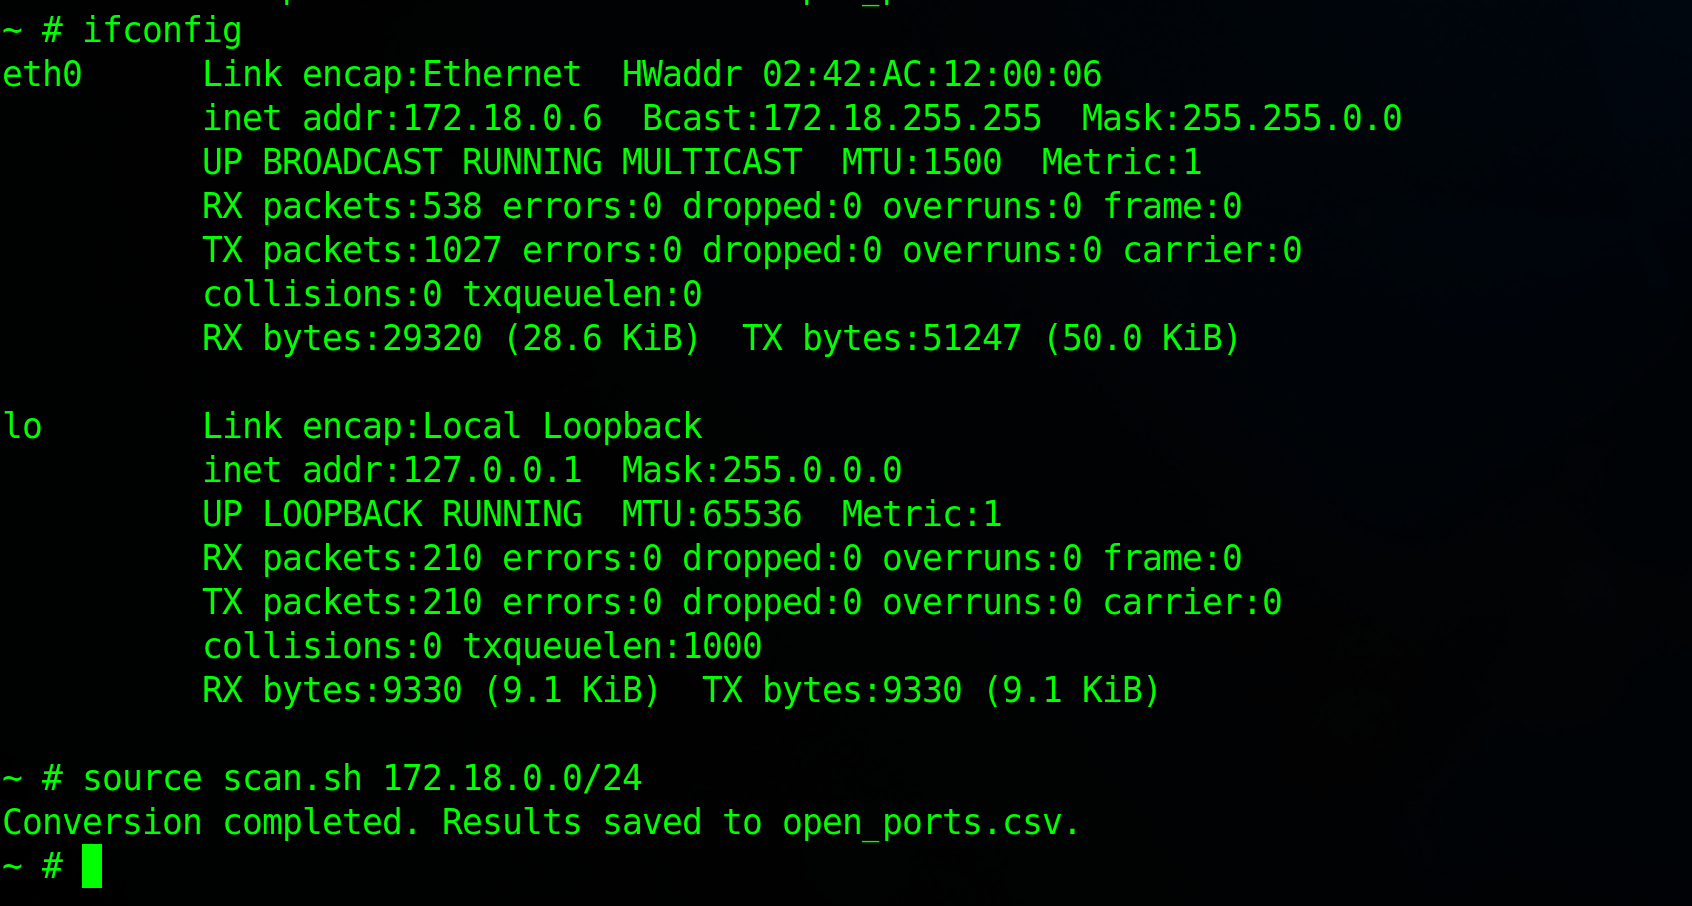
\includegraphics[scale=0.2]{images/scan_sample.png}
\end{figure}


\begin{figure}[hbtp]
\caption{خروجی دادن پورت‌های اسکن شده در فرمت csv}
\centering
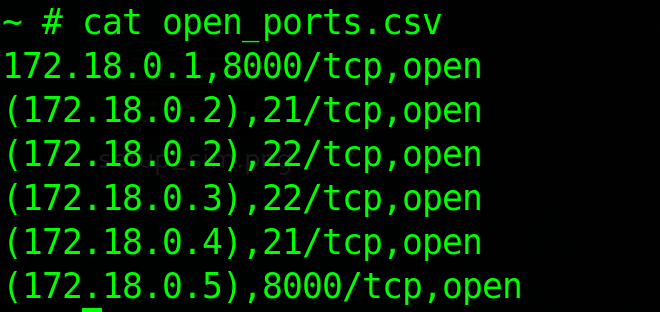
\includegraphics[scale=0.2]{images/open_ports.png}
\end{figure}



\begin{figure}[hbtp]
\caption{شروع حمله با اجرای اسکریپت hack.sh}
\centering
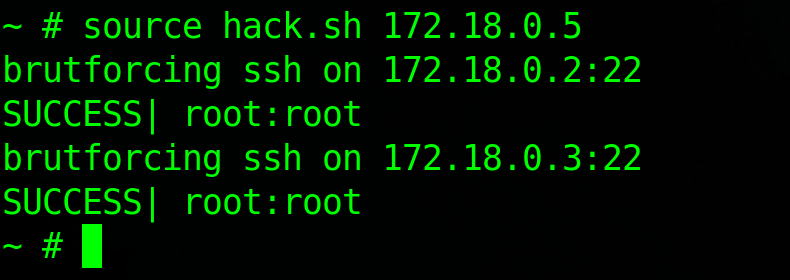
\includegraphics[scale=0.2]{images/hack_sample.png}
\end{figure}
سپس فایل hack.sh را اجرا کرده و ip وب سرور را به آن به عنوان ورودی بدهید. با این کار حمله آغاز می‌شود و شما در صفحه دیتا بیس وب سرور میتوانید مشاهده کنید که هر یک دقیقه یک بار، اطلاعات امنیتی سرورهای قربانی برای شما ارسال و در دیتابیس ذخیره می‌شوند.

\begin{figure}[hbtp]
\caption{لاگ‌های وب سرور پس از شروع حمله}
\centering
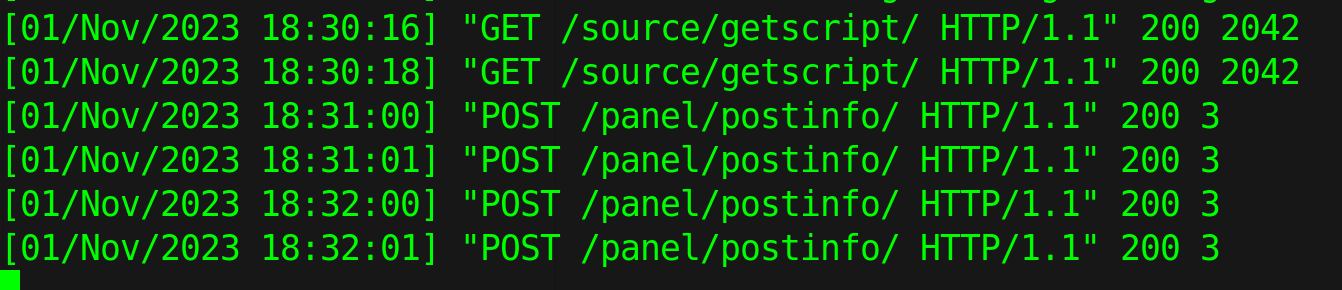
\includegraphics[scale=0.2]{images/web_server_logs.png}
\end{figure}

\begin{figure}[hbtp]
\caption{اطلاعات ارسال شده توسط سرورهای قربانی به صورت رکورد در دیتابیس ذخیره می‌شوند}
\centering
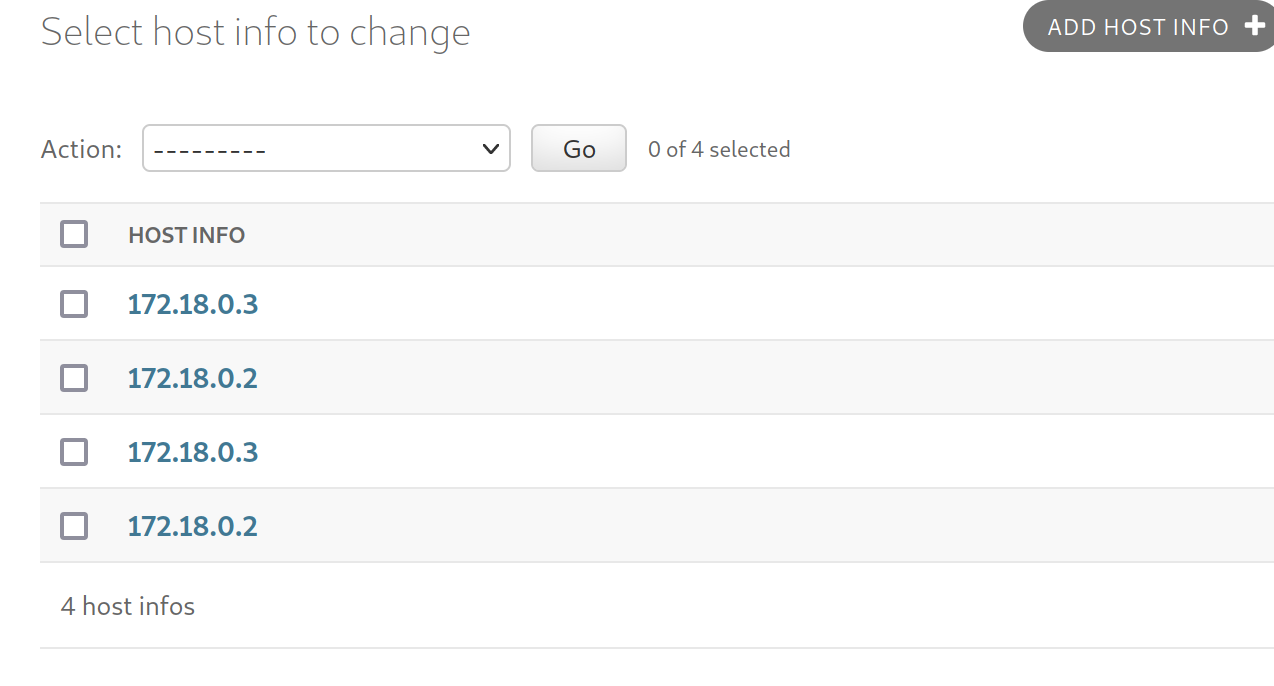
\includegraphics[scale=0.2]{images/DB_panel.png}
\end{figure}


\subsection{حذف کانتینرها و شبکه داکر}
در نهایت برای حذف شبکه داکر ساخته شده و متوقف کردن کانتینرهای در حال اجرا، اسکریپت remove\_containers.sh را اجرا کنید.


\section{گیتهاب پروژه}
برای مشاهده ریپازتوری گیتهاب پروژه می‌توانید از \href{https://github.com/mohammad-osoolian/Network-Security-Project}{این لینک} استفاده کنید. همچنین در صورت نیاز می‌توانید هر کدام از image ها را مستقیما از داکرهاب دانلود یا مشاهده کنید:

\begin{itemize}
    \item \href{https://hub.docker.com/r/mohammad2782/attack-machine}{attack machine image}
    \item \href{https://hub.docker.com/r/mohammad2782/web-server}{web server image}
    \item \href{https://hub.docker.com/r/mohammad2782/target-server}{target server image}
\end{itemize}

\end{document}